
%(BEGIN_QUESTION)
% Copyright 2006, Tony R. Kuphaldt, released under the Creative Commons Attribution License (v 1.0)
% This means you may do almost anything with this work of mine, so long as you give me proper credit

Design a thermistor circuit that produces an increasing output voltage with increasing temperature.  Hint: the topology of the circuit may be as simple as this:

$$\includegraphics[width=15.5cm]{i00042x01.eps}$$

You will need to choose which resistor ($R_1$ or $R_2$) to make the thermistor and which to make fixed, and also choose which type of temperature coefficient the thermistor will have (either {\it positive} or {\it negative}).  After making these choices and drawing your circuit below, explain how it works (i.e. what happens to all the voltages and currents as temperature increases):

\vfil 

\underbar{file i00042}
\eject
%(END_QUESTION)





%(BEGIN_ANSWER)

This is a graded question -- no answers or hints given!

%(END_ANSWER)





%(BEGIN_NOTES)

Either make $R_1$ the thermistor with a {\it negative} temperature coefficient, or make $R_2$ the thermistor with a {\it positive} temperature coefficient.

%INDEX% Measurement, temperature: thermistor circuit

%(END_NOTES)


